JavaScript was introduced 1995 with the intention to solve small tasks such as validation of input data and small animations \parencite{Moller2018} and is today well supported in virtually all web browsers on both desktop and mobile \parencite{Zakai2011}. According to \textcite{TiwariSolihin2012} more than 95\% of all web pages are viewed with JavaScript enabled web browsers and more than 99\% of all web sites use JavaScript. While web apps have an advantage of portability compared to native mobile apps, the dynamic typing and prototypes features of JavaScript makes it execution inefficient \parencite{ParkJungMoon2015}.

\subsubsection*{Optimizations}

Figure \ref{reference-architecture} illustrates a reference architecture of a web browser developed by \textcite{GrosskurthGodfrey2005}. The component in a web browser that is focused on JavaScript interpretation and execution is called a JavaScript engine \parencite{JeonChoi2012}. The last few years manufacturers of web browsers has been focused on optimizing JavaScript performance through just-in-time (JIT) and recently ahead-of-time (AOT) compilation \parencite{HerreraChenLavoieHendren2018}.

\begin{comment}

\begin{figure}[!h]
\centering
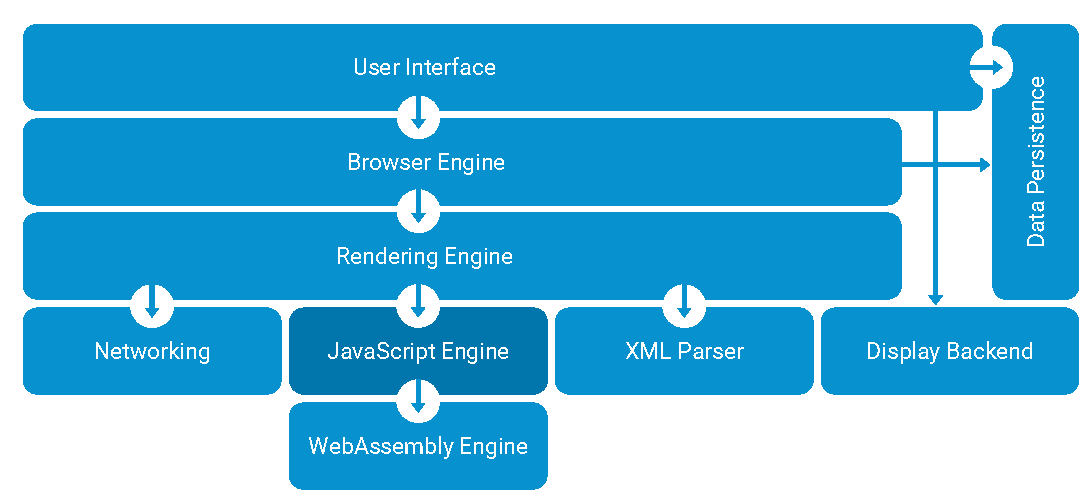
\includegraphics[width=16cm,keepaspectratio]{../Figures/reference-architecture}
\caption{Web browser reference architecture. Adapted from \textcite{GrosskurthGodfrey2005}.}
\label{reference-architecture}
\end{figure}
    
\begin{figure}[!h]
\centering

\includegraphics[width=16cm,keepaspectratio]{../Figures/javascript-optimization}
\caption{JavaScript execution tiers. Adapted from \textcite{ParkKimMoon2017,ZhuykovVardanyanMelnikBuchatskiySharygin2015}.}
\label{javascript-optimization}
\end{figure}
    
\end{comment}

% Previously we had characters/strings being parsed into an abstract syntax tree (AST) that was then used to generate bytecode that was run with an interpreter.

The way that JavaScript has been managed has changed with time. The first tier (Figure \ref{javascript-optimization}) is concerned with doing realtime interpretation and from that creating bytecode that is executed \parencite{ParkKimMoon2017}. Before browser vendors saw a competitive in having a really fast JavaScript engine the first tier was the only job of the JavaScript engine. The introduction of the second tier, the JIT compilation step gave JavaScript performance a real boost. In some browsers there are as many as four different optimization levels within the JIT compilation step based on the number of times a certain piece of code is executed. \textcite{ZhuykovVardanyanMelnikBuchatskiySharygin2015} and others are currently experimenting with AOT compilation where JavaScript is actually compiled ahead of time which exchanges faster performance for larger size.

%optimizations starts with looking at the execution and generate optimized versions of the course, this is called just in time compliations. some browsers (safari) has up to 4 levels of optimizations. not a good optimized. webassembly needs this.

%https://blog.mozilla.org/luke/2014/01/14/asm-js-aot-compilation-and-startup-performance/

%parse, compile + optimize, re-optimize, execute, garbage collection

% https://hacks.mozilla.org/2017/02/what-makes-webassembly-fast/

%- the web has become the most ubiquitous application platform ever, and yet by historical accident the only natively supported programming language for that platform

%- a new portable size and load-time-efficient format suitable

%''One popular way of accelerating JavaScript is using the just-in-time compilation (JITC), which translates the JavaScript source code to the machine code at runtime. Unfortunately, JavaScript JITC for web apps suffers from the parsing and compilation overhead seriously, which offsets the performance gain of executing the compiled code.'' \parencite{ParkJungMoon2015}

%A major problem with optimizing is that fact that JavaScript is a loosely typed language, which means that the interpreter needs to be able to store any type of data in any variable. If the interpreter instead would be able to distinguish between which type of data each variable can store, it would be much easier to optimize. This is asm.js.

\subsubsection{TypeScript}

TypeScript is a superset of JavaScript that adds type information \parencite{DeWolffHage2017}. Type information allows the programmer to see mistakes sooner during the development phase rather than later in runtime. In Listing \ref{listing:typescript} the JavaScript function \texttt{isPrime} has been enhanced with type information.

\lstinputlisting[label=listing:typescript,language=JavaScript,caption=prime.ts]{../Listings/isprime.ts}

Before TypeScript is published as part of a web site it is transformed to regular JavaScript using the TypeScript compiler (tsc). This does thus not directly solve the problem of performance, but decreases the number of runtime errors, and enables future backend optimizations such as improved guesses by the JIT-compiler. TypeScript also comes with a toolchain that allows JavaScript developers to write better JavaScript.

% if there should be any subsubsection section shown in the table of contents it should be asm.js

\subsubsection{asm.js}

Another approach to optimize JavaScript is asm.js. Asm.js i subset of JavaScript focused on performance \parencite{Zakai2018}. If the browser understands asm.js it will skip certain steps in the JavaScript engine designed to optimize ''normal'' JavaScript, as it knows that asm.js is already optimized in certain ways. JavaScript engines that does not understand asm.js simply parses the JavaScript as usual as all asm.js scripts are valid JavaScript. \textcite{Zakai2018} describes the idea behind asm.js as removing the dynamic and complex parts of JavaScript and thus ending up with a subset that is more easily optimized by the JavaScript engine.

\lstinputlisting[label=listing:asmjs,language=JavaScript,caption=asm.js]{../Listings/asm.js}
%\listing[abc]{../Listings/isprime.ts}
%\listing[Some listing caption]{asm.js}
%\figure[Some figure caption]{javascript-optimization}
%\lstinputlisting[label=prototype,language=JavaScript,caption=prototype.js]{../Listings/prototype.js}

Listing \ref{listing:asmjs} shows an implementation of a C string calculation length function written in asm.js containing two prominent differences between asm.js and regular JavaScript. 

On line 2, 6, and 8 a bitwise operator \texttt{|0} is used. The operator has no effect on the value of the result but provides a hint to the JavaScript engine that the result is of the type signed integer which can be used by the JavaScript engine to optimize the performance. 

The use of \texttt{MEM8[]} on line 5 is another way to increase the performance in asm.js. In asm.js much of the memory is written to and read from a type buffer instead of relying on the slower garbage collector provided by the JavaScript engine.

Asm.js is not meant to be written by hand but rather serve as compilation target. The tool EmScripten \parencite{Zakai2011} was created as a source-to-source compiler between other languages such as C/C++ and asm.js. As asm.js is a subset of JavaScript all browsers that can run JavaScript can run asm.js code that has been created by the EmScripten tool.

This enhancement lead to the notion of some calling asm.js and sometimes JavaScript as the assembly language of the web. However, JavaScript as the assembly language of the web is not very good. JavaScript was famously invented in 10 days and was never designed as a compilation target.

\textcite{HaasRossbergSchuffTitzerHolmanGohmanWagnerZakaiBastien2017} notes that while the web has given rise to demanding web apps JavaScript as a language, being the only programming language available in web browsers, is not very well equipped to support such applications. \textcite{ReiserBlaser2017} describes that there is always a desire for higher performance in web applications and \textcite{Zakai2018} describes JavaScript (asm.js included) as an obstacle for demanding high-performing apps.


%- if the browser understands "use asm" it skips many of the optimization steps. it it doesnt it simply ignores it. 
%asm.js is pretty verbose and thus has some overhead.

%- memory in both asm.js and webassembly is a continious array of bytes. the webassembly array is actually shared with javascript so you can read and write to it from both languages

%- works as a stack machine in a assembly language

%- module interchangeable

%- show examles in node? its available since node 8

%- working with strings are harder 17m

% https://www.youtube.com/watch?v=pBYqen3B2gc

%- a stack machine 4 types, 67 instructions. designed to support streaming compilation, simple validation rules. exports / imports functions. shared linear memory with javascript